\documentclass[12pt]{amsart}
\usepackage{graphicx} % Required for inserting images
\usepackage{amsmath}
\usepackage{hyperref}

\title{Fourier Analysis}
\author{Henry Jacobs}
\date{April 2025}

\begin{document}
\maketitle

\section{Bell-ringer (5 minutes)}
With your group come up with the most random sentence you possibly can.

Example: {\it ``She used her own hair in the soup to give it more flavor''}


\section{Introduction}
So far we have looked at power series, which can be thought of as sums (possibly infinite) of multiples of $x^k$.
Today we will consider Fourier series which are sums of multiples of $\sin(kx)$ and $\cos(kx)$.
Explicitly, a {\bf Fourier series is a series of the form}

$$
S(x) = \underbrace{\sum_{k=0}^{\infty} c_k \cos(kx) }_{\text{even component}}
+ \underbrace{\sum_{k=1}^{\infty} s_k \sin(kx)}_{\text{odd component}}
$$

Where the $c_k$'s and $s_k$'s are coefficients.

\section{Fourier Approximations}
Consider the function 
$$
f(x) = \begin{cases}
    1 & \text{for } 0 < x < \pi \\
    -0.5 & \text{for } -\pi < x \leq 0
\end{cases}
$$

We are not able to approximate this function with a Maclauren series because it is discontinuous at $x=0$.
We can not approximate it with a Taylor series very well either.
The Taylor series centered at any $c < 0$ is the constant function $P(x) = \frac{-1}{2}$ and for $c > 0$ the Taylor approximation is the constant function $P(x)=1$. 

However, we can approximate $f$ as a Fourier series pretty well though

$$
   f(x) = \frac{1}{4} + \frac{3}{\pi} \sum_{n=0}^{\infty} \frac{\sin((2n+1)x)}{2n+1} 
$$

The $20$th order Fourier expansion is plotted against $f(x)$ in figure \ref{fig:fourier} on page \pageref{fig:fourier}.  The Desmos code can be accessed at \url{https://www.desmos.com/calculator/rtnbrdojzh}

\begin{figure}
    \centering
    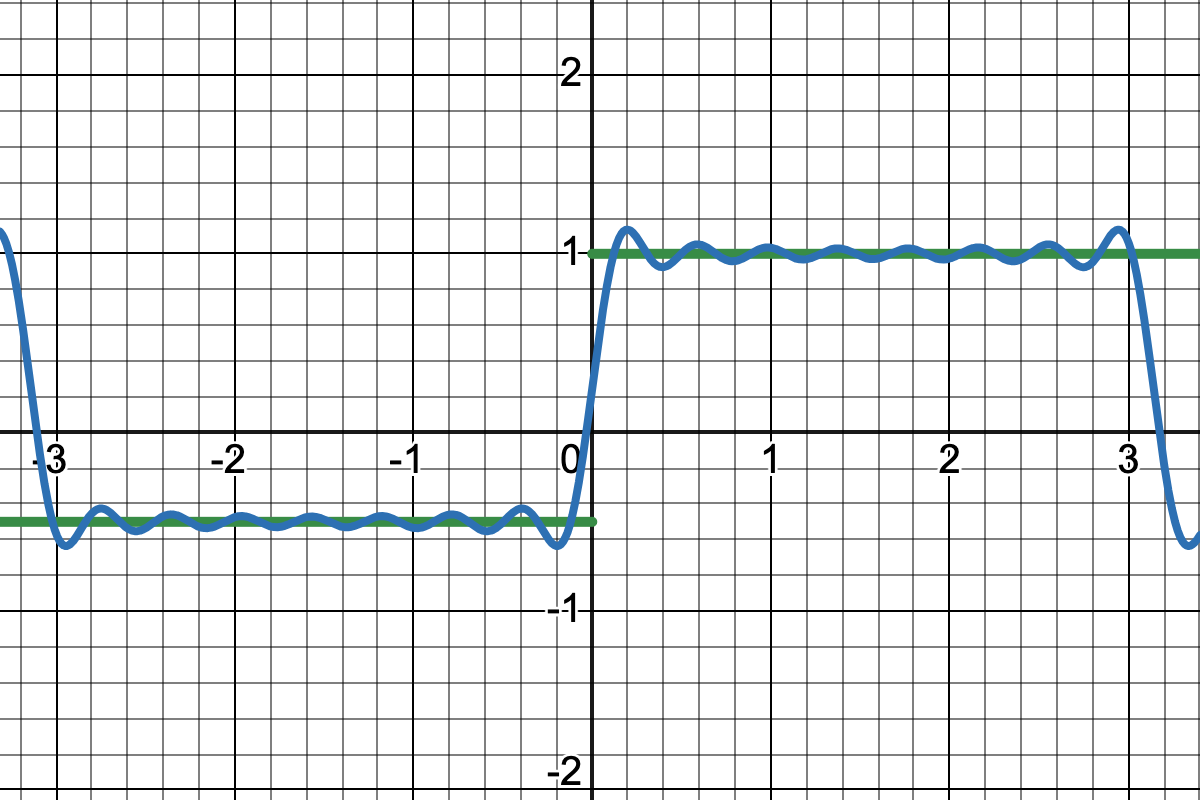
\includegraphics[width=0.5\textwidth]{./images/desmos-graph.png}
    \caption{7th order Fourier approximation of a step function}
    \label{fig:fourier}
\end{figure}


\subsection{The Fourier Transform}
If you are given a piecewise continuous function, $f(x)$, then how should
you approximate $f(x)$ as a Fourier series?

The answer is {\bf the Fourier Transform}. 
Explicitly, you can compute the coefficients

\begin{align}
c_0 &= \frac{1}{2\pi} \int_{-\pi}^\pi f(x) dx\\
c_k &= \frac{1}{\pi} \int_{-\pi}^\pi f(x) \cos(kx) dx \\
s_k &= \frac{1}{\pi} \int_{-\pi}^\pi f(x) \sin(kx) dx
\end{align}
for $k=1,2,3,\dots, N$ and you would find that

$$
f_N(x) = \sum_{k=0}^{N} c_k \cos(kx) + \sum_{k=1}^{N} s_k \sin(kx)
$$
is a good approximation of $f(x)$ for large $N$.

Formally, this means that 
$$
  f(x) = \lim_{N \to \infty} f_N(x)
$$
for all $x \in [-\pi, \pi]$ except at the discontinuities.


\section{Practice Problems}

\subsection{Problem 1}
Consider the function $f(x) = x$ on the domain $[-\pi, \pi]$.
Compute a 6th order Fourier approximation of this function.
In other words: compute $c_0, c_1, c_2, \dots c_6$ as well as $s_1, s_2, \dots, s_6$.

BONUS:  Compute the coefficient $s_k$ and $c_k$ for arbitrary $k$.

\subsection{Problem 2}
Assume we are given a Fourier series
$$
    q(x) = \sum_{k=0}^{\infty} c_k \cos(kx) + \sum_{k=1}^{\infty} s_k \sin(kx)
$$

What is the Fourier series of $\frac{dq}{dx}$?

What is the Fourier series of $\frac{d^2q}{dx^2}$?

\end{document}
